% !TEX root=../index.tex
\chapter{Kinect}
\label{chap:Kinect}

Ad onor del vero, ciò che viene comunemente chiamato \emph{sensore di profondità} (o sensore di distanza) del Kinect, è in realtà uno \emph{scanner 3D a luce strutturata}\footnote{Nonostante ciò, lo si continuerà a chiamare \emph{sensore di profondità}, leggermente inesatto, ma decisamente più breve ed intuitivo}.
\begin{wrapfigure}{R}{0cm}
    \centering
    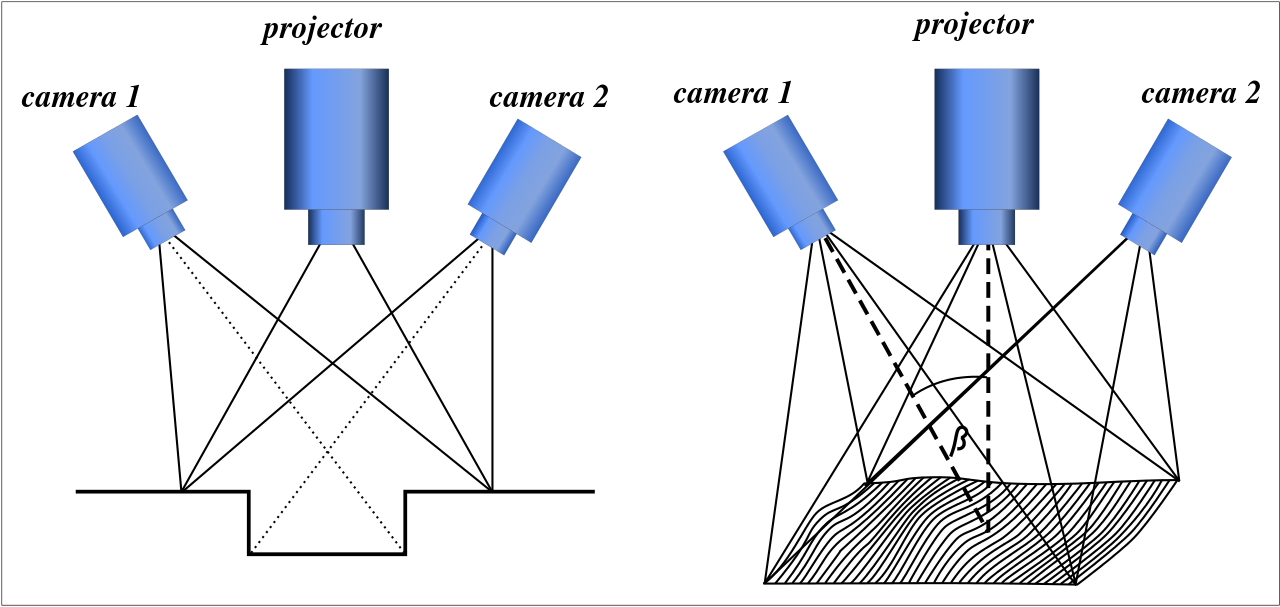
\includegraphics[width=8cm]{img/3d-structured-light-scanner.png}
    \label{fig:structured_light_scanner}
    \caption{Schematizzazione di uno scanner 3D a luce strutturata.}
\end{wrapfigure}
Un sorgente di raggi infrarossi proietta una serie di pattern codificati. La deformazione indotta dalle superfici degli oggetti interessati viene acquisita da una o più telecamere ed utilizzata per il calcolo delle coordinate tridimensionali.

Il risultato di un sensore di questo tipo è un insieme di triplette $(x,y,z)$, organizzate in una \emph{immagine di profontità}, una struttura dati che è molto simile ad una semplice immagine in scala dei grigi, dove il valore di ogni pixel rappresenta la misura in millimetri della distanza della superficie dal sensore.
La forte somiglianza con le immagini in scala dei grigi è supportata dal fatto che ogni pixel è codificato utilizzando 16bit.

La massima affidabilità del sensore del Kinect si ha per distanza comprese tra $50cm$ e $4,5m$.
Il dispositivo è montato al soffitto a $2,8m$ da terra e ha un campo visivo di $70^{\circ} \times 60^{\circ}$, il quale, all'altezza del pavimento, determina un'area di cattura di circa $4m \times 5m$.

La dimensione di ogni immagine di profondità è di $512 \times 424$ pixel. Nativamente non vengono codificate in alcun modo particolare, sono delle semplici matrici di interi.
Il Kinect V2 è in grado di catturarne fino a 30 al secondo. Utilizzando un apposito software di registrazione è stato possibile mettere insieme dei video di profondità a 30 fps.
